%%%%%%%%%%%%%%%%%%%%%%%%%%%%%%%%%%%%%%%%%

\documentclass{article}
\usepackage[a4paper, total={6in, 10in}]{geometry}

\usepackage[version=3]{mhchem} % Package for chemical equation typesetting
\usepackage{siunitx} % Provides the \SI{}{} and \si{} command for typesetting SI units
\usepackage{graphicx} % Required for the inclusion of images
\usepackage{natbib} % Required to change bibliography style to APA
\usepackage{amsmath} % Required for some math elements 
\usepackage{comment} % Comment package 
\setlength\parindent{0pt} % Removes all indentation from paragraphs
\renewcommand{\labelenumi}{\alph{enumi}.} % Make numbering in the enumerate environment by letter rather than number (e.g. section 6)
\usepackage{subfigure} % Subfigure plotting
\setlength{\parindent}{2em}
\usepackage[justification=centering]{caption} % Center the figure caption

%----------------------------------------------------------------------------------------
% Title Page
%----------------------------------------------------------------------------------------

\title{Evaluation of Early Stage Startup Success Using Investor Rankings \& Founders Background} % Title

\author{Thomas E. J. Moxham \& Yigit Ihlamur} % Author name

\date{\today} % Date for the report

\begin{document}

\maketitle % Insert the title, author and date

\begin{abstract}
\noindent Results from the project MoneyBall which evaluates the likelihood of start up success are presented. Features are engineered from two datasets based on the founders background and the company investors. A description of how these features are extracted and an analysis of their underlying distribution is also given. These features are used as the input data for two classification models which predict the true success ratio better than random chance. A discussion of the most suitable metrics for evaluating success and the future direction the project could take is also provided.
\end{abstract}

%----------------------------------------------------------------------------------------
% Introduction
%----------------------------------------------------------------------------------------

\section{Introduction}

Vela partners is a firm using machine learning and data analytics to access the likelihood of start up success and make informed investment decisions. Predicting future outcomes in early-stage investing is much more difficult than other investment fields due to the limited availability of quantitative data and only qualitative, typically categorical features provided. The goal of this project is given two labelled datasets of successful and unsuccessful companies can we make more probable predictions of the likelihood of a companies success than random chance. To achieve this we combine features extracted from the MoneyBall dataset itself with recent results from the Midas Touch project which scores investors. The report is organized as follows, in section \ref{sec:feature_generation} we describe how features are engineered and extracted from the datasets. In section \ref{sec:finitial_statistical_analysis} an initial statistical analysis is performed on the features to understand the underlying relationships and determine which are best suited for the final model. In section \ref{sec:model_evaluation} we evaluate the trained models are evaluated discuss the best metrics for achieving this are discussed. Finally in section \ref{sec:conclusion_outlook} results are discussed and we conclude with the possible future directions the project could take.

%----------------------------------------------------------------------------------------
% Feature Generation
%----------------------------------------------------------------------------------------

\section{Feature Generation}
\label{sec:feature_generation}

MoneyBall and Midas Touch are the two datasets provided and are used to engineer the founder and investor features respectively, therefore we will discuss them each in turn. The MoneyBall dataset is of primary interest and consists of two spreadsheets containing successful and unsuccessful software companies. Successful here is defined as a company with a valuation greater than \$500M and unsuccessful is defined as have raised less than \$10M in investment in the last 5 years. The success column is labelled as a binary integer of 1 for successful and 0 for unsuccessful. The structure of each set is identical\footnote{With the exception of a few the domain, success type and blah features in successful companies which are not used within the project or report.} and lists rows of companies with columns with company attributes given below. The combined successful and unsuccessful dataset contains approximately 44k rows, however many features are missing so a periodically dropped as features of interest are engineered and described better in the proceeding sections. The exact columns of interest and used for feature generation are described in greater detail in the proceeding section. 

\begin{itemize}
	\item[]\textbf{MoneyBall Columns:} Founded year, country code, city, category list, category group list, university of founders, degree of founders, subject degree of founders, gender of founders, city of founders, previous companies of founders, prev titles of founders, investor names, short description and long description.
\end{itemize}

\subsection{Founder Features}

One of the most challenging aspects with the MoneyBall dataset is that it is categorical whereas out model requires a single numerical input. Based on previous work the founders university and previous companies were found to be good features for predicting the successfulness of companies so were chosen to complement and compare with the investor features discussed next. A list of all the founders universities were mapped to their respective world ranking using the QS world university rankings 2022 data-set and then features generated from this list. Missing entries and universities which did not feature on the QS world ranking list were populated with the average value of the that column. Instances of the previous companies attended by founders were used to generate the top most popular previous companies. The success rate of previous companies attended by founders was  found as the ratio of successful to unsuccessful instances, including only companies with at least 50 former employees.

\begin{itemize}
	\item\textbf{Average founders university score:} The sum of all founders respective university scores divided by the total number of universities in the list, null university scores were set to the mean column value.
	
	\item\textbf{Maximum founders university score:} The maximum university score out of all the founders university scores, null university scores were disregarded and were set to the mean column value.
	
	\item\textbf{Minimum founders university score:} The minimum university score out of all the founders university scores, null university scores were disregarded and were set to the mean column value.
	
	\item\textbf{Most popular previous company:} A list of the 10 most poplar previous founder employers was found by counting the instances of each company. This is a binary category set too true if any of the founders was previously employed at one of the companies listed below.  

	Companies: Google, Microsoft, Meta, Yahoo, Apple, Techstars, IBM, Oracle, Accenture, Cisco
	
	\item\textbf{Most Successful previous company:} A list of the most successful previous previous founder employers generated by taking the ratio of successful to unsuccessful instances and selecting those with a success ratio greater than 50\% and having at least 25 former employees. This is a binary category set too true if any of the founders was previously employed at one of the companies.  
	
	Companies: Seres Therapeutics, Joule Unlimited Technologies, Axcella, Flagship Pioneering, Harvard Medical School, Harvard Business School, Genentech, Tesla, Massachusetts Institute of Technology, University of California Berkeley

	\item\textbf{MoneyBall previous company:} Category based on whether the founders were previously employed at a company within MoneyBall dataset itself. If the previous company was successful (as labelled by MoneyBall) then the feature is categorized as 1, if it was unsuccessful (as labelled by MoneyBall) its categorized as -1 and if it didn't feature its categorized as 0. There were around 2.6k MoneyBall companies out of the 44k dataset which previously employed founders of other companies. 
		
\end{itemize}

\subsection{Investor Features}

Previous interns on the MoneyBall project reported investor information providing a high correlation with the successfulness of companies. This led to its own dedicated study appropriately named "Midas Touch", which ranks smaller lesser known investors against a core set of "brand name" investors which are known to choose successful companies. The ranking encompasses a number of features including the "brand name" list of investors, the investor name, the number of companies they've invested in and similar investors but overall results in a normalized investor score from zero to one. This dataset was utilized by mapping the investor name in the MoneyBall dataset to their respective scores in the Midas dataset. An additional column with "brand name" investors removed was also generated. Start ups with either no investor information or investors which which did not feature in the Midas dataset were dropped. The Midas Touch dataset contained investor scores for around 10k investors, after dropping rows without investor information from the MoneyBall dataset this left around 7.6k rows. From the list of investor scores a number of investor metrics were generated and detailed below.

\begin{itemize}
	\item\textbf{Overall number of investors:} Simply counts the total number of unique investors\footnote{The same investor may appear multiple times in a companies investor list where they have entered at multiple funding stages.} in a company and is normalized by the maximum value in the column. In the long term as more companies are added a dynamic normalization routine would be required.
	\item\textbf{Average investor score:} The sum of all unique investor scores divided by the total number of unique investors.
	
	\item\textbf{No brand name investors average score:} The sum of all unique investor scores with "brand name" investors removed divided by the total number of unique investors with "brand name" investors removed.
	
	\item\textbf{Maximum investor score:} The maximum investor score out of all unique investor scores.
	
	\item\textbf{No brand name investors maximum score:} The maximum investor score with "brand name" investors removed out of all unique investor scores with "brand name" investors removed.
	
	\item\textbf{Minimum investor score:} The minimum investor score out of all unique investor scores.
	
	\item\textbf{No brand name investors minimum score:} The minimum investor score with "brand name" investors removed out of all unique investor scores with "brand name" investors removed.

\end{itemize}

%----------------------------------------------------------------------------------------
% Initial Statistical Analysis
%----------------------------------------------------------------------------------------

\section{Initial Statistical Analysis}
\label{sec:finitial_statistical_analysis}

We use exploratory data analysis to summarize the main characteristics of the dataset and better understand what the data can tell us beyond the formal modeling or hypothesis testing task. Our first realization is that the MoneyBall dataset does not contain the same proportion of successful and unsuccessful cases but is split roughly 17\% to 83\% for the two datasets. This has ramifications on how we should evaluate our final model and is discussed in the next section. All proceeding analysis of is shown in Fig. \ref{fig:founder_statistics} and Fig. \ref{fig:investor_statistics} for the founder and investors features respectively. Firstly the underlying data distribution is computed for the university scores of the founders and the investors scores. This shows a clear trend that start ups are more likely to be started by founders who attended highly ranked universities. The large proportion of zero scores likely arises because mappings between the university scores and names could not be found due to a different spelling rather than as a true characteristic of the dataset. The investor distributions for all investor scores shows a secondary peak at investor scores at 1 corresponding to the "brand name" investor scores in the set, this is dealt with by removing dropping "brand names" from the set and results in a much more normal distribution.

To select the best features for our final model we employ a univariate analysis using the probability density function (PDF) of the features: continuous data is best visualized with histograms which categorical discrete data is best visualized with bar charts. In general the most significant features will have PDF curves with different shapes and a large separation for the successful and unsuccessful target variables. From the university scores none of the features display much separation, we observe that the average and maximum scores display the greatest difference in shape. Founders which previously worked at one of the the most popular companies had little impact on the successfulness of the company, however founders which worked at a previously successful company shows a considerable increase in the likelihood of success. Finally founders which previously worked at an unsuccessful MoneyBall company has little to no impact on the successfulness, however if founders worked at a successful MoneyBall company this appears to increase the successfulness of the company. The PDF curves of the average and maximum investor scores show the most difference in shape and seperation for both the complete and no "brand name" investor cases. The minimum investor scores for the complete and no "brand name" investors are the same and show little difference in shape or separation between the two distributions.

%----------------------------------------------------------------------------------------
% Model Evaluation
%----------------------------------------------------------------------------------------

\section{Model Evaluation}
\label{sec:model_evaluation}

As both the combined successful and unsuccessful datasets are highly imbalanced the usual accuracy metric is not good enough to evaluate the machine learning models and features. Therefore we require the precision and recall metrics which are better suited to evaluating the models ability to identify True positives, i.e the models ability to accurately predict successful companies which is of greater interest. The precision and recall are defined below,
\begin{equation}
	\textrm{Precision}=\frac{\textrm{True Positives (TP)}}{\textrm{True Positives (TP)}+\textrm{False Positives (FP)}}
\end{equation}
\begin{equation}
	\textrm{Recall}=\frac{\textrm{True Positives (TP)}}{\textrm{True Positives (TP)}+\textrm{False Negatives (FN)}}
\end{equation}
A system with high recall but low precision returns many results, but most of its predicted labels are incorrect when compared to the training labels. A system with high precision but low recall is just the opposite, returning very few results, but most of its predicted labels are correct when compared to the training labels. An ideal system with high precision and high recall will return many results, with all results labeled correctly. Therefore we are most interested in generating models with both high precision and recall, but precision should take priority.

All features discussed previously where used to generate 3 feature groups which included only founder features, only investor features and the combination of both. These were split into stratified training and testing sets in order to keep the proportion of successful and unsuccessful dataset constant in both. Four common classification models were tested including the Random Forests (RF), K-Nearest Neighbors (KNN), Support Vector Machine (SVC) and Gradient Boosting Classifier (GBC), hyper-parameters were manually optimized for each and SVC and GBC produced the most interesting results so were focussed on. Models were validated using a k-fold cross-validation, whereby the dataset was split k times into training and testing sets and for each split the model is trained and tested. As the True precision-recall ratio is whats most of interest to use, these curves are plotted for each fold as shown in Fig. \ref{fig:svc_model} and Fig. \ref{fig:gbc_model} in order to validate the results. In addition to this the importance of each feature can be extracted from the GBC model and is shown in Fig. \ref{fig:gbc_features} for the combines feature set.

All the tested models clearly show a precision greater than 17\% which correspond to a higher accuracy than random chance in predicting successful companies; the main difference between the models is how this value changes with the recall. The founder features clearly show consistently high precision amongst the folds with low recall, i.e the founder features can predict successfulness very accurately and consistently on a small portion of the dataset, this is mostly visually observable in the SVC figure. Investor features have a lower overall precision but work over a much larger recall range i.e the investor feature can predict successfulness over a greater portion of the dataset with a slightly lower precision. Additionally the initial ratios for smaller recalls are much more varied across the folds but converge for larger recalls, this is mostly visually observable in the GBC figure. The combined feature set appears to incorporate the benefits of each feature set, with more consistent ratios across the folds, and higher recalls for both small and large recall ranges. It is important to note these curves vary with different train test splits but the general behavior described has been observed to remain. The overall model accuracy for the combined feature set was found to be around 82\% across all models which agrees well with previously reported results using similar features.

%----------------------------------------------------------------------------------------
% Conclusions & Outlook
%----------------------------------------------------------------------------------------

\section{Conclusions \& Outlook}
\label{sec:conclusion_outlook}

The final models achieve a high accuracy but more importantly a high precision recall ratio for successful datasets. Some of the more notable conclusions are that the max investor score for all investor scores as well as the "brand name" investor scores removed has the highest significance on the company success. This suggest having a single high scoring investor in the company is a significant indicator of a start up's future success. Additionally the fact that the max investor score with "brand name" investors removed is the second most impactful feature has the potential to offer a significant edge in choosing companies, even when "brand name" investors have not invested. A single figure of merit of the model accuracy is difficult to assign as the precision recall ratio can be modified depending on the future project direction. One possibility is using a model with a relatively low precision ($\sim0.4$) but large recall ratio ($\sim0.8$) as an initial filtering stage on a large dataset composed of millions of companies, resulting in a large number of predictions with a relatively low accuracy. Alternatively a model with a relatively high precision ($\sim0.8$) but low recall ratio ($\sim0.05$) could be applied on a smaller dataset composed of a few thousand companies to generate very accurate signals of a few companies. One conclusion that can be drawn is that for the combined feature across all recall ratios set is the precision greater than random chance, which was one of the fundamental aims of the project. Below a few comments are given on the future directions other projects may take. 

\begin{itemize}

	\item The use of other classification models including neural networks, as well as hyper-parameter optimization using method such as random search of the existing models. It was observed during the project that the hyper-parameters play an important role in the behavior of the model and can change the outcomes quite drastically.
	
	\item A key component of this research was the use of the Midas Touch results, this can be regarded as an independent dataset that shows high correlation with company success. The generation of features based on a companies successfulness label (as was performed here) can not be regarded as truly independent and may introduce unknown biases. Further projects accessing other attributes such as the founders university and education and previous employers that generate independent datasets are likely to yield more concrete results.
	
	\item A better encoding method that accounts for null or missing results rather than dropping rows or simply using the mean value, this is important as the datasets frequently contain missing or null data. 
	
	\item A greater analysis of the resulting classification models. This includes identifying where there are outliers and better refining our method of feature engineering, in universities for example many rows are mis/unlabelled as the mappings between the two datasets is difficult to achieve. Additionally understanding the underlying fundamentals between the precision recall ratio could further provide insights into how it may be improved in the future. Finally reducing/permuting the list of features to see how this effects results.
	
	\item Repeating the analysis with different Midas Touch parameters, in this report we used a dataset based on investor scores with at least 10 or more previous investments, which results in a large investor dataset and increases the instances of rows. Another dataset which considers investors with 30 or more previous investments will yield fewer rows, but may be more precise. There is the option to also alter the number and names of the "brand name" investors with which the scores are generated.
	
\end{itemize}




%----------------------------------------------------------------------------------------
% Figures
%----------------------------------------------------------------------------------------

\pagebreak

% Founder Statistics
\begin{figure}[h]
	\centering
	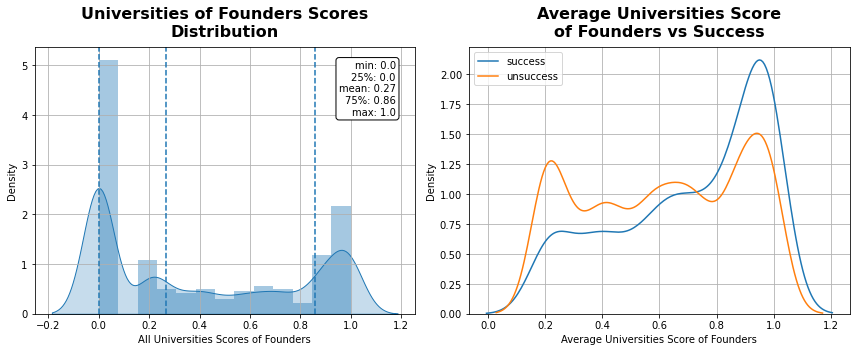
\includegraphics[width=0.8\textwidth]{figures/university_distribution_average_score}
	\subfigure[]{
		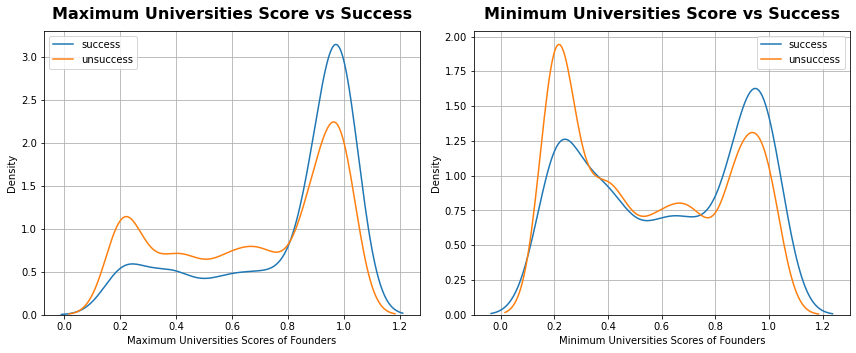
\includegraphics[width=0.8\textwidth]{figures/university_max+min_vs_success}}	
	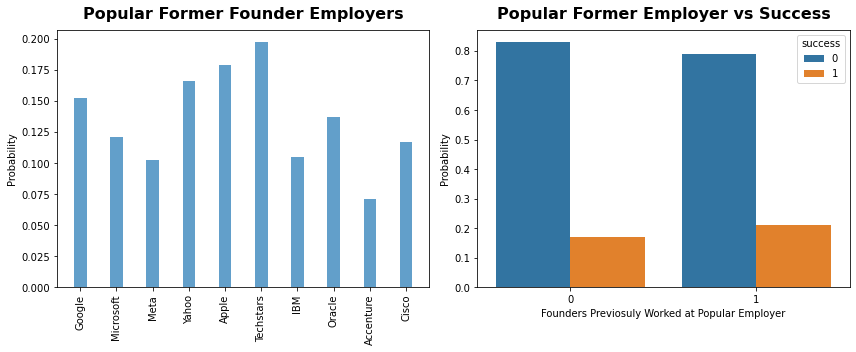
\includegraphics[width=0.8\textwidth]{figures/employer_popular_popoluar_vs_success}
	\subfigure[]{
		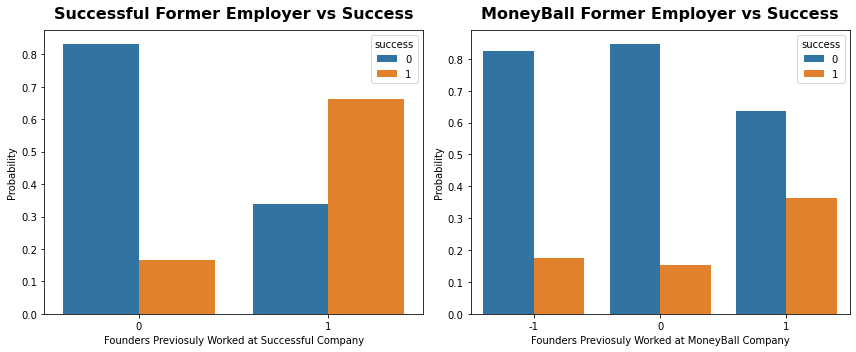
\includegraphics[width=0.8\textwidth]{figures/employer+moneyball_vs_success}}
	\caption{Statistical analysis of (a) the Founders university background based on the corresponding universities QS world ranking score and (b) the founder former employer.}
	\label{fig:founder_statistics}
\end{figure}

% Investor Statistics
\begin{figure}[h]
	\centering
	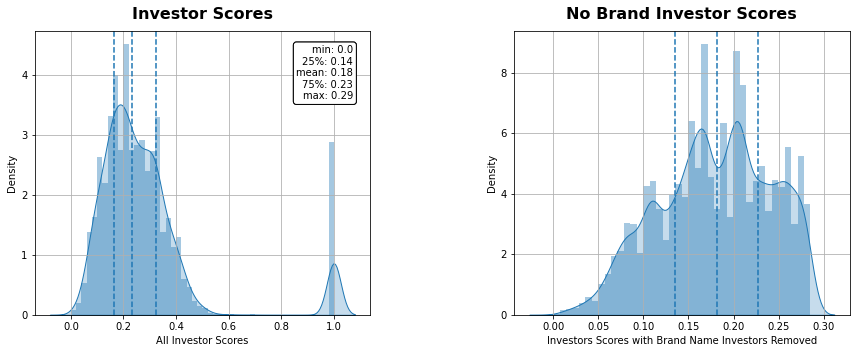
\includegraphics[width=0.8\textwidth]{figures/investor+nobrand_scores_distribution}
	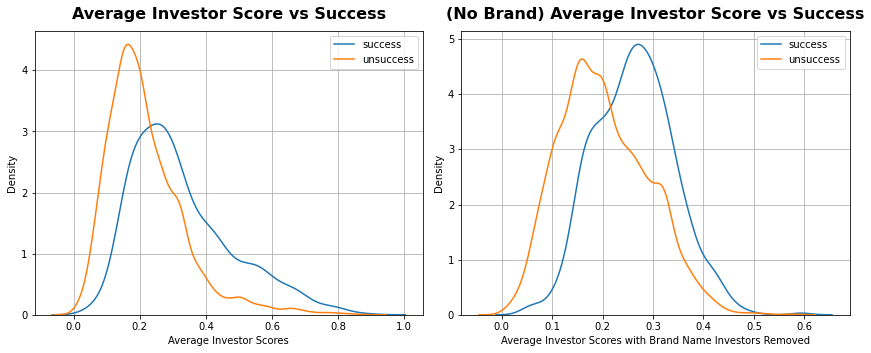
\includegraphics[width=0.8\textwidth]{figures/investor+nobrand_average_vs_success}
	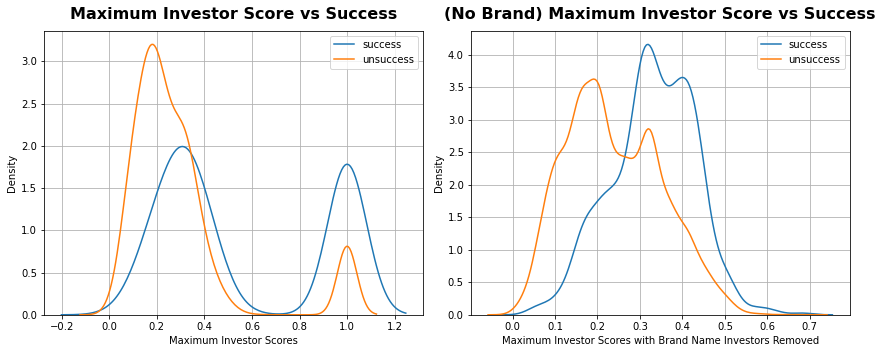
\includegraphics[width=0.8\textwidth]{figures/investor+nobrand_max_vs_success}
	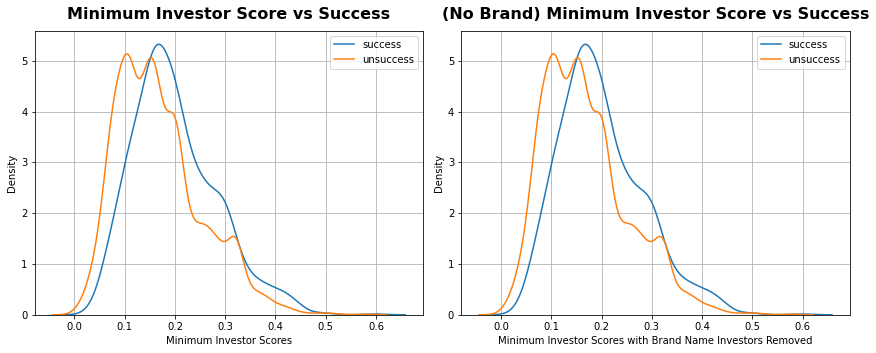
\includegraphics[width=0.8\textwidth]{figures/investor+nobrand_min_vs_success}
	\caption{Statistical analysis of investor scores based on the Midas dataset.}
	\label{fig:investor_statistics}
\end{figure}

% SVC Model
\begin{figure}[h]
	\centering
	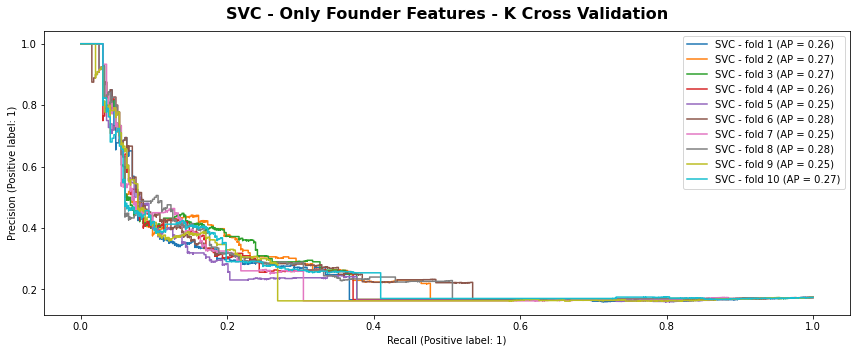
\includegraphics[width=\textwidth]{figures/svc_cfounder_kcross}
	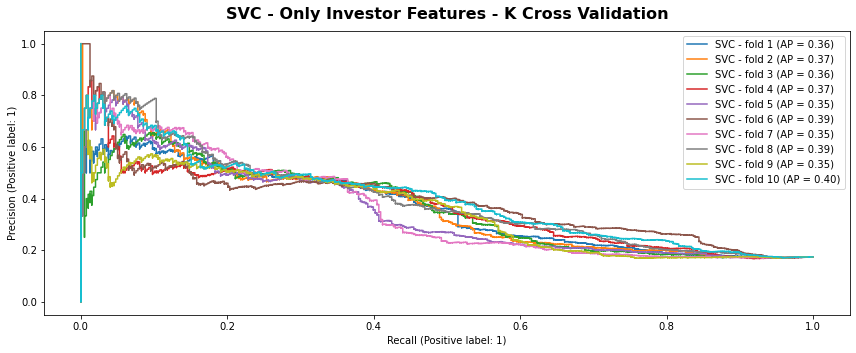
\includegraphics[width=\textwidth]{figures/svc_investor_kcross}
	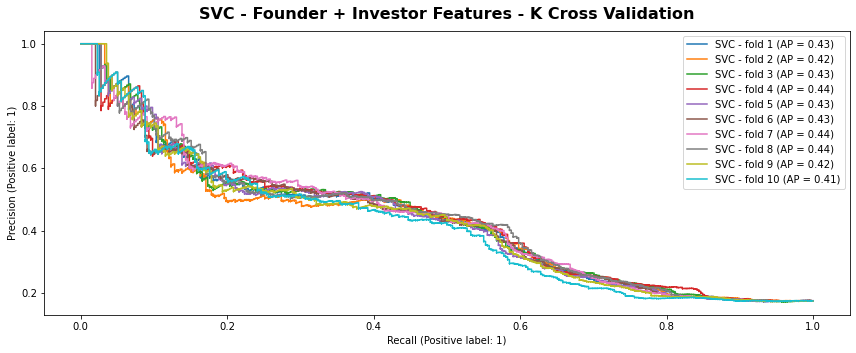
\includegraphics[width=\textwidth]{figures/svc_combined_kcross}
	\caption{The SVC model results for the founder, investor and combined feature sets, the curves are the True precision recall ratio and were repeated with k-folds to validate the results. AP is the average precision for its respective curve.}
	\label{fig:svc_model}
\end{figure}

% GBC Model
\begin{figure}[h]
	\centering
	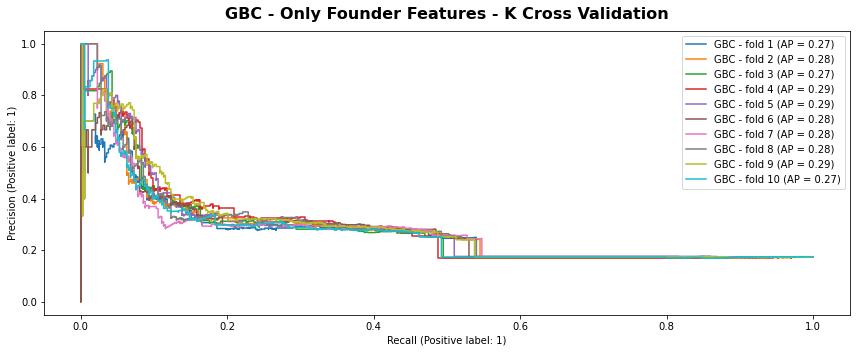
\includegraphics[width=\textwidth]{figures/gbc_founder_kcross}
	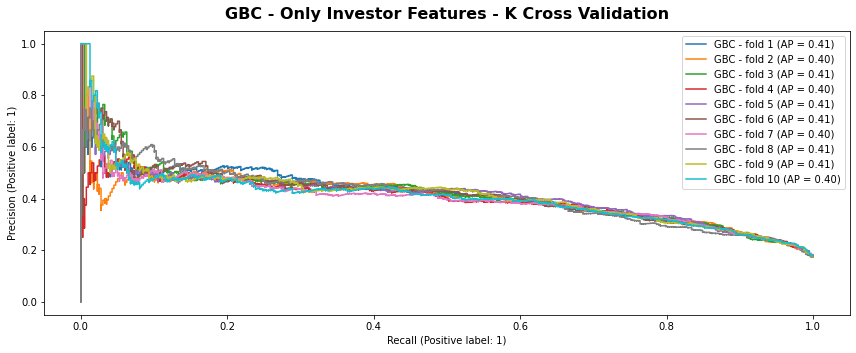
\includegraphics[width=\textwidth]{figures/gbc_investor_kcross}
	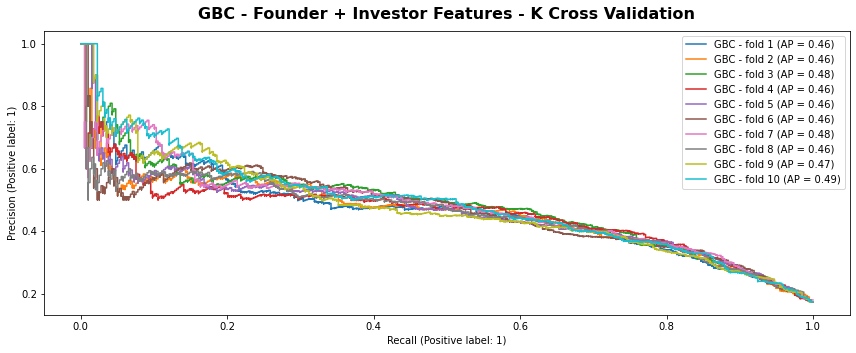
\includegraphics[width=\textwidth]{figures/gbc_combined_kcross}
	\caption{he GBC model results for the founder, investor and combined feature sets, the curves are the True precision recall ratio and were repeated with k-folds to validate the results. AP is the average precision for its respective curve.}
	\label{fig:gbc_model}
\end{figure}

% GBC Features
\begin{figure}[h]
	\centering
	\caption{The most important features for the combined feature set trained on the GBC model.}
	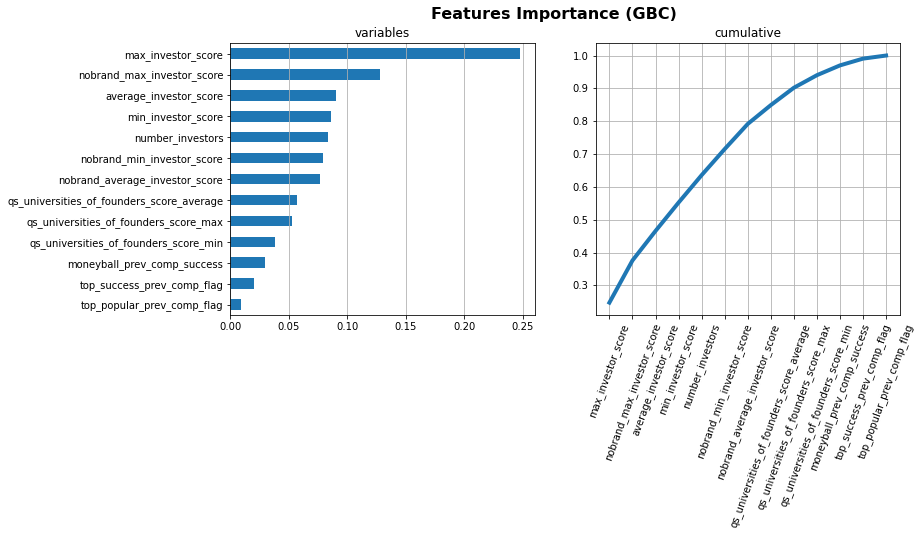
\includegraphics[width=\textwidth]{figures/gbc_feature_analysis}
	\label{fig:gbc_features}
\end{figure}




















\end{document}